\documentclass[10pt]{article}
\usepackage[polish]{babel}
\usepackage[utf8]{inputenc}
\usepackage[T1]{fontenc}
\usepackage{amsmath}
\usepackage{amsfonts}
\usepackage{amssymb}
\usepackage[version=4]{mhchem}
\usepackage{stmaryrd}
\usepackage{graphicx}
\usepackage[export]{adjustbox}
\graphicspath{ {./images/} }

\title{LIGA MATEMATYCZNA im. Zdzisława Matuskiego LISTOPAD 2019 SZKOŁA PODSTAWOWA klasy VII - VIII }

\author{}
\date{}


\begin{document}
\maketitle
\section*{ZADANIE 1.}
Wyznacz takie cyfry \(a, b, c\), że \(\overline{a a a}+b=\overline{b c c c}\). Symbol \(\overline{x y z}\) oznacza liczbę trzycyfrową zapisaną w dziesiętnym systemie pozycyjnym.

\section*{ZADANIE 2.}
Cztery koleżanki z wakacji: Ania, Basia, Daria i Ela kupiły sukienki. Każda mieszka w innym mieście i każda kupiła sukienkę w innym kolorze. Odgadnij, w jakim mieście mieszka każda z koleżanek oraz jaki jest kolor jej sukienki, jeżeli:

\begin{itemize}
  \item sukienka Ani nie jest czerwona;
  \item dziewczyna w zielonej sukience nie mieszka w Słupsku;
  \item Basia ma białą sukienkę, ale nie mieszka w Gdańsku;
  \item dziewczynka w czerwonej sukience mieszka w Lęborku;
  \item Daria mieszka w Bytowie, a jej sukienka nie jest niebieska.
\end{itemize}

\section*{ZADANIE 3.}
Wyznacz wszystkie liczby naturalne co najmniej dwucyfrowe, które maleją jedenastokrotnie po skreśleniu cyfry jedności.

\section*{ZADANIE 4.}
Przy dzieleniu liczb \(a, b\), \(c\) przez 5 otrzymujemy odpowiednio reszty 1, 2, 3. Podaj reszte z dzielenia sumy kwadratów tych liczb przez 5.

\section*{ZADANIE 5.}
Czworokąt podzielono przekątnymi na cztery trójkąty. Pola trzech z nich podane są na rysunku. Oblicz pole szarego trójkąta.\\
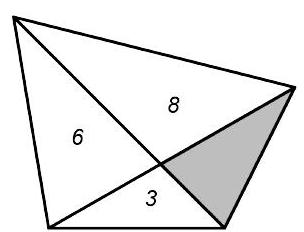
\includegraphics[max width=\textwidth, center]{2024_11_21_ad1a2131fc305a932f44g-1}


\end{document}